\subsubsection{Package sequenziatore::client::ipresenter::iuser::ilogic}
\begin{figure}[H] \centering 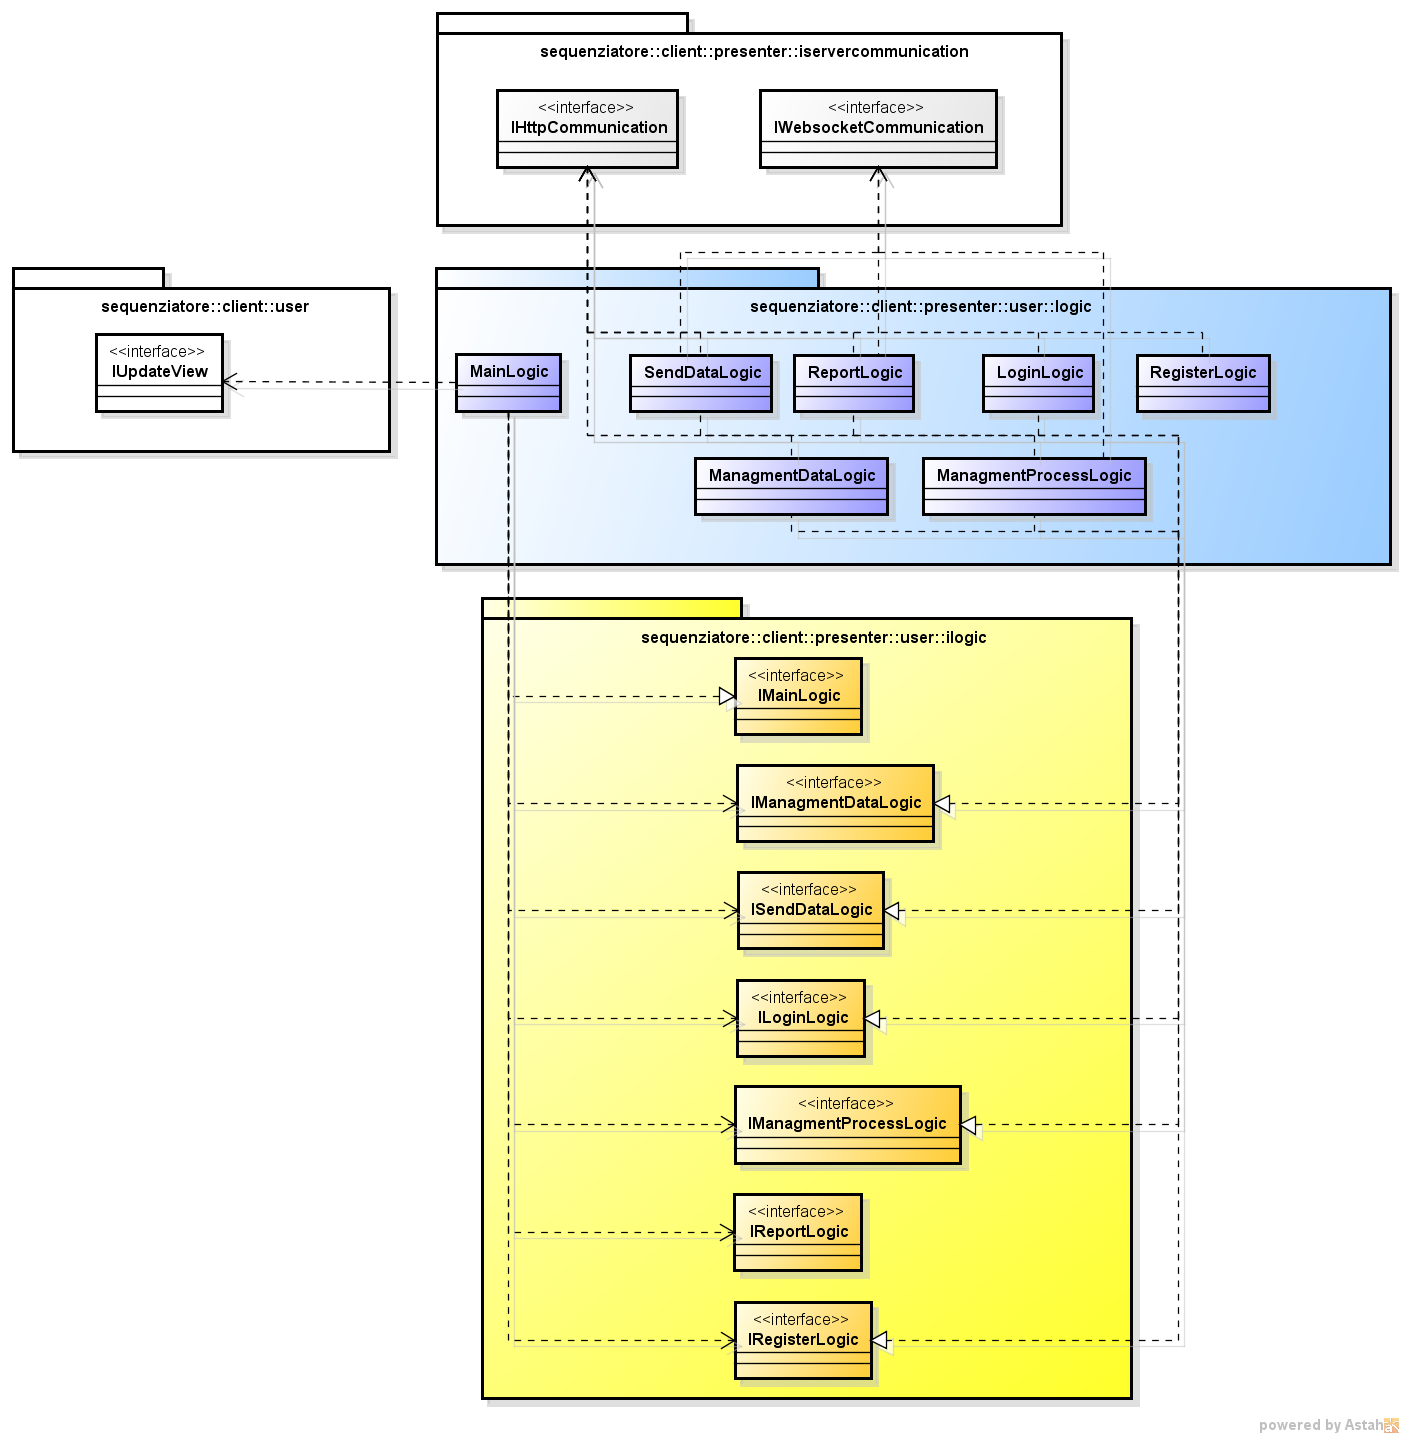
\includegraphics[width=%
\textwidth]
{./pack/presenter_user.png} \caption{Diagramma presenter user}
\end{figure}
\paragraph{IMainLogic}
\begin{itemize}
\item \textbf{Nome:} \texttt{IMainLogic};
\item \textbf{Package:} \texttt{\iLogicUser{}};
\item \textbf{Descrizione:} Interfaccia che permette di gestire gli eventi generati dalla componente \textit{View}.
\end{itemize}

\paragraph{ILoginLogic}
\begin{itemize}
\item \textbf{Nome:} \texttt{ILoginLogic};
\item \textbf{Package:} \texttt{\iLogicUser{}};
\item \textbf{Descrizione:} Interfaccia che ha il compito di gestire le richieste di autenticazione e chiusura della sessione da parte dell'utente.
\end{itemize}

\paragraph{IRegisterLogic}
\begin{itemize}
\item \textbf{Nome:} \texttt{IRegisterLogic};
\item \textbf{Package:} \texttt{\iLogicUser{}};
\item \textbf{Descrizione:} Interfaccia che ha il compito di gestire le richieste di registrazione da parte dell'utente.
\end{itemize}

\paragraph{IManagmentDataLogic}
\begin{itemize}
\item \textbf{Nome:} \texttt{IManagmentDataLogic};
\item \textbf{Package:} \texttt{\iLogicUser{}};
\item \textbf{Descrizione:} Interfaccia che ha il compito di gestire la visualizzazione e la modifica dei dati dell'utente.
\end{itemize}

\paragraph{IManagmentProcessLogic}
\begin{itemize}
\item \textbf{Nome:} \texttt{IManagmentProcessLogic};
\item \textbf{Package:} \texttt{\iLogicUser{}};
\item \textbf{Descrizione:} Interfaccia che ha il compito di gestire e accedere alle informazioni relative allo stato dei processi.
\end{itemize}

\paragraph{ISendDataLogic}
\begin{itemize}
\item \textbf{Nome:} \texttt{ISendDataLogic};
\item \textbf{Package:} \texttt{\iLogicUser{}};
\item \textbf{Descrizione:} Interfaccia che ha il compito di gestire l'inserimento e l'invio di dati da parte degli utenti.
\end{itemize}

\paragraph{IReportLogic}
\begin{itemize}
\item \textbf{Nome:} \texttt{IReportLogic};
\item \textbf{Package:} \texttt{\iLogicUser{}};
\item \textbf{Descrizione:} Interfaccia che ha il compito di gestire la creazione di report sull'andamento dei processi in esecuzione.
\end{itemize}